
\documentclass{article}
\usepackage{array,ragged2e}
\usepackage{graphicx}
\usepackage[top=2cm, bottom=3cm,right=1cm, left=1cm, headsep=26pt]{geometry}
\usepackage[T1]{fontenc}
\usepackage{sidecap}
\usepackage{helvet}
\renewcommand{\familydefault}{\sfdefault}

% used in maketitle
\title{Evaluacion 2}
\author{Castillo Bastida Eduardo\\
Departamento de Fisica \\
Universidad de Sonora}
\date{01 de diciembre de 2017}


% Enable SageTeX to run SageMath code right inside this LaTeX file.
% documentation: http://mirrors.ctan.org/macros/latex/contrib/sagetex/sagetexpackage.pdf
% \usepackage{sagetex}

\begin{document}
\maketitle
\clearpage

\section{Actividad 1: Describir el ejemplo}
El programa del ejemplo, se le da un valor "n" y "x" ya escogidos (20 y 1.0 respectivamente). Con estos datos se calcula mediante una Serie de Maclaurin el exponencial del valor de x en una funcion. En el programa se le otroga valores ya elegidos y te arroja el resultado del exponencial calculado, imprimiendo el exponencial verdadero con el comando de "exp(x)" y ya se compara el error entre el exponencial que calculamos en la función que es muy aproximado.

\clearpage
\section{Actividad 2: Exponente}
\begin{verbatim}
!
!! Taylor.f90
!! 
!! Made by (Eduardo Castillo Bastida)
!! Login   <batman@ltsp165.example.com>
!! 
!! Started on  Fri Dec  1 10:45:16 2017 Eduardo Castillo Bastida
!! Last update Time-stamp: <2017-dic-01.viernes 14:30:54 (batman)>
! ----------- Begin ------------

program Taylor

    double precision, dimension (15) :: f
	integer :: i, j, n
	double precision, dimension (100)   :: x, y, exp_real
	double precision :: fi, fj, term, partial_sum

     open (1, file = 'datos.dat', status = 'unknown')
	
	do n=1, 15, 2
	do i=0, 100, 1
	  fi = dble(i)
	  fi = fi / 10.0d0
	call exptaylor (nmax, j, fi, fj, y)
	exp_real(n) = y(n)
	write(1,*) fi, exp_real(n)

	end do
	write (1,*) ' '
	end do
     close (1)


end program Taylor

!====================================
subroutine exptaylor(nmax, j, fi, fj, y)
!====================================

  ! argumentos de la subrutina:
  integer, intent (in) :: nmax
  double precision, intent (in) :: fi
  integer ::j
  double precision, dimension (100), intent (out) :: y
  double precision ::fj, nterm, partial_sum


    term = 1.
    partial_sum = nterm

    do j=1,nmax
       ! El termino #j es  x**j / j! que es el termino anterior (x10 x/j):
       fj=dble(j)
       nterm = fi/fj   
        ! Sumamos este termino al anterior:
        partial_sum = partial_sum + nterm
        end do
     nterm = j       ! numero de terminos utilizados
     y = partial_sum  ! Este es el valor regresado
end subroutine exptaylor
\end{verbatim}
\clearpage

\begin{figure}
  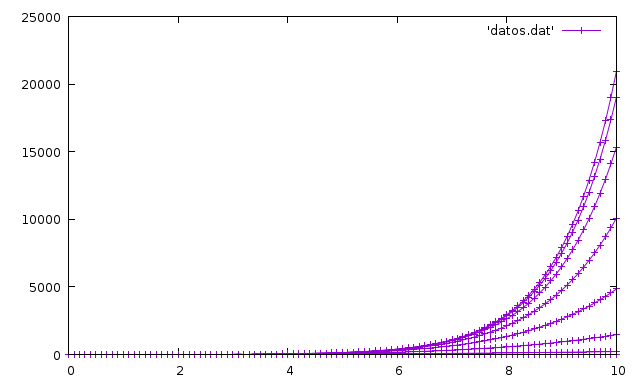
\includegraphics[width=\linewidth]{Full.png}
  \caption{Grafica completa de los valores aproximados de exp(x)}
\end{figure}


\section{Actividad 3: Seno}
\begin{verbatim}

!! CaculoSeno.f90
!! 
!! Made by (Eduardo Castillo Bastida)
!! Login   <batman@ltsp165.example.com>
!! 
!! Started on  Fri Dec  1 14:57:30 2017 Eduardo Castillo Bastida
!! Last update Time-stamp: <2017-dic-01.viernes 15:02:06 (batman)>

program CalculoSeno
	double precision, dimension (10000) :: f, x, sen, y
	integer :: i, j, n
	double precision :: fi, fj, term, partial_sum, sign, pot, fact
	

     open (1, file = 'senos.dat', status = 'unknown')
	fi = -3.1d0
	do i=1, 60
	write (1,*) fi, fi
	fi = fi + 0.1d0
	
end do

	write (1,*) ' '
	do n=1, 15, 2
	  fi = -3.1d0
	do i=1, 60
	fi = fi + 0.1d0
	call seno (n, j, fi, fj, sen, sign, pot, fact)
	y(n) = sen(n)
	write (1,*) fi, y(n)

	end do
	write (1,*) ' '
	end do
     close (1)

   end program CalculoSeno

   subroutine seno (n, j, fi, fj, sen, sign, pot, fact)
	integer, intent (in)      :: n
	double precision, intent (in) :: fi
	integer :: j
	double precision, dimension (10000), intent(out) :: sen
	double precision :: fj, term, partial_sum, sign, pot, fact

	
	sign = 1.0d0
	term = fi
	partial_sum = term
	pot = fi
	fact = 1
	do j = 1, n
	 fj = dble(j)
	 pot = fi**(j + 2)
	 fact = fact * (j + 1) * (j + 2)
	 sign = sign * (-1.0d0)
	 term = pot / fact
	 term = term * sign
	 partial_sum = partial_sum + term
	 sen(j) = partial_sum
	 
	end do

	 
end subroutine seno
\end{verbatim}
\clearpage
\begin{figure}
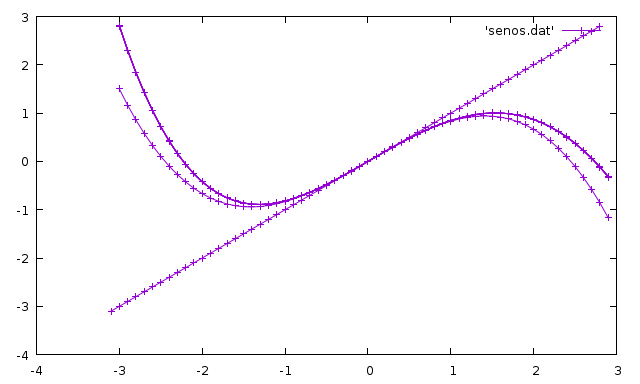
\includegraphics[width=\linewidth]{Seno.png}
\caption{Grafica del seno verdadero (la recta)y las graficas de las aproximaciones}
\end{figure}


\end{document}
